\section{Architecture du projet}

\subsection{Un système client/serveur}

Au premier semestre de cette année, notre étude bibliographique nous a permis d'étudier les deux systèmes de fenêtrages majeurs sous linux, X Window System (implémentation X.org) et le tout jeune Wayland.
Cette étude nous a permis de décider de calquer notre futur système de fenêtrage (Pron) sur X Window System qui était selon nous, le plus simple et le plus adapté.
De plus, l'implémentation X.org étant un projet mûr, il est très bien documenté et les solutions conceptuelles qu'il a utilisé sont validées et fonctionnent.

Notre système de fenêtrage sera divisé en deux grandes parties : le serveur graphique en tant que tel, Pron, et la librairie client implémentant le protocole de communication Pron, la pronlib.

Après avoir étudié les solutions existantes pour ce qui est de la gestion des fenêtres, nous avons opté pour un système inspiré de Metacity.
Le gestionnaire de fenêtres, Guacamole, sera un client à part entière du serveur graphique (Pron), qui se contentera d'intercepter certains événements comme on le verra plus tard.

Enfin, la librairie de widgets, Sombrero, s'inspirera à la fois de Qt (en version 4), et de gtkmm (wrapper pour GTK+).

Voici un schéma illustrant les différents acteurs de notre architecture et leurs dépendances.
On peut voir que la PronLib est le cœur de notre système.
Elle est utilisée par tous les éléments pour communiquer avec Pron et Pron l'utilise également pour communiquer avec les clients.
  
\begin{figure}[H]
  \centering
  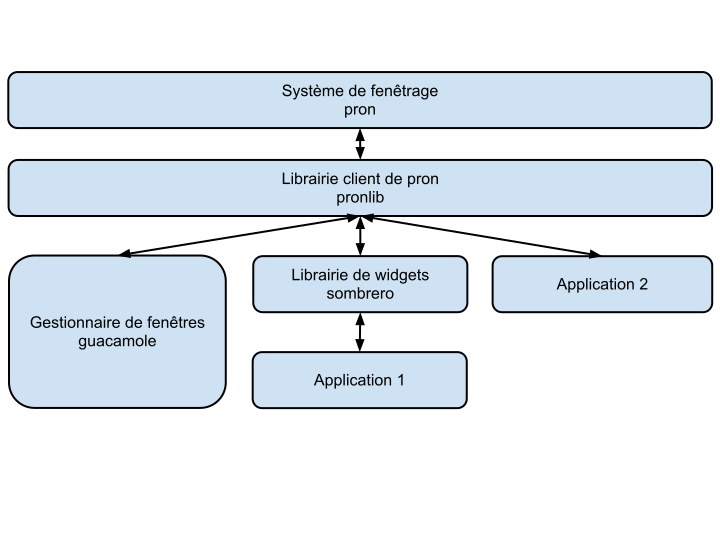
\includegraphics[width=14cm]{images/architecture.png}
  \caption{Architecture}
  \label{fig:architecture}
\end{figure}

On remarque que Guacamole utilise directement la PronLib.
C'est le cas au moment de la rédaction de ce rapport mais il sera bientôt réimplémenté avec la librairie Sombrero.

\subsection{Langage de programmation}

Pour ce projet, nous avons décidé d'utiliser le C++ pour de nombreuses raisons :

\begin{itemize}
  \item Langage orienté objet : la COO\footnote{Conception Orientée Objet} est très agréable notamment pour une librairie de widgets
  \item Langage compilé : pas besoin d'environnement d'exécution comme Java qui n'est pas disponible sous TacOS
  \item Facile à intégrer à un projet en C (TacOS étant codé en C)
  \item Performances
  \item Langage connu et apprécié par les membres de l'équipe
  \item Langage offrant des fonctionnalités très bas niveau
  \item Langage permettant l'héritage multiple
\end{itemize}